\section{Products}
    \subsection{REST API}
        \begin{frame}[t]{Developing the REST API}\framesubtitle{Overview}
            \begin{itemize}
                \item Focus on the next generation of GIRAF developers
                \begin{itemize}
                    \item Documentation
                    \item Design
                \end{itemize}
                \item Synchronisation
                \item Security
            \end{itemize}
        \end{frame}

        \begin{frame}[t]{Developing the REST API}\framesubtitle{Our contributions}
            Sprints 3-4:
            \begin{itemize}
                \item Pictograms
                \item Sequences
                \item Week Schedules
            \end{itemize}
            \bigskip
            Differences from developing Apps.
            \begin{itemize}
                \item Unit Tests
                \item Linting
                \begin{itemize}
                    \item Saved time during code--review
                    \item Enforced a code--style
                \end{itemize}
                \item Strict(er) code--review
            \end{itemize}
        \end{frame}
\subsubsection{Pictograms}
\begin{frame}[t, fragile]{Example of the REST API in use}\framesubtitle{Creating a new pictogram}
To create a pictogram:\\
Request: \\
\texttt{POST /department/\{id\}/pictogram/}
\begin{lstlisting}[language=json]
{
  "title" : "Test",
  "ownerId" : 1337,
  "departmentId" : 2,
  "accessLevel" : "PROTECTED"
}
\end{lstlisting}
Response:
\begin{lstlisting}[language=json]
{
  "type": ".Pictogram",
  "id": 8,
  "lastEditAt": "2016-06-19 11:36:09",
  "title": "Test"
}
\end{lstlisting}
\end{frame}
\begin{frame}[t, fragile]{Example of the REST API in use}\framesubtitle{Creating a new pictogram cont.}
Request: \\
\texttt{PUT /department/\{id\}/pictogram/8/} \\
With the PNG as data (Content-Type: image/png).
Response:
\begin{lstlisting}[language=json]
{
  "type": ".Pictogram",
  "id": 8,
  "lastEditAt": "2016-06-19 11:36:29",
  "title": "Test"
}
\end{lstlisting}
Then: \\
\texttt{GET /department/\{id\}/pictogram/7/image} \\
will return the pictogram.
\end{frame}


    \subsection{GIRAF--Apps}
        \begin{frame}[t]{GIRAF--Apps}
            Sprints 1-2:
            \begin{itemize}
                \item Gradle issues
                \item PictoSearch library
                \item Week Schedule
            \end{itemize}
        \end{frame}


        \subsubsection{Gradle}
            \begin{frame}[t]{GIRAF--Apps}\framesubtitle{The Gradle Build System}
                \begin{itemize}
                    \item Fixing the initial broken library builds.
                    \item Assisting with Jenkins.
                    \item Helping various groups with small issues.
                \end{itemize}
            \end{frame}

        \subsubsection{PictoSearch}
            \begin{frame}[t]{GIRAF--Apps}\framesubtitle{PictoSearch}
                \begin{itemize}
                    \item Improving the initial view.
                    \item \enquote{real--time} search.
                \end{itemize}
                \bigskip
                \only<1| handout:1>{
                Old view:
                \begin{figure}[htb]
                    \centering
                    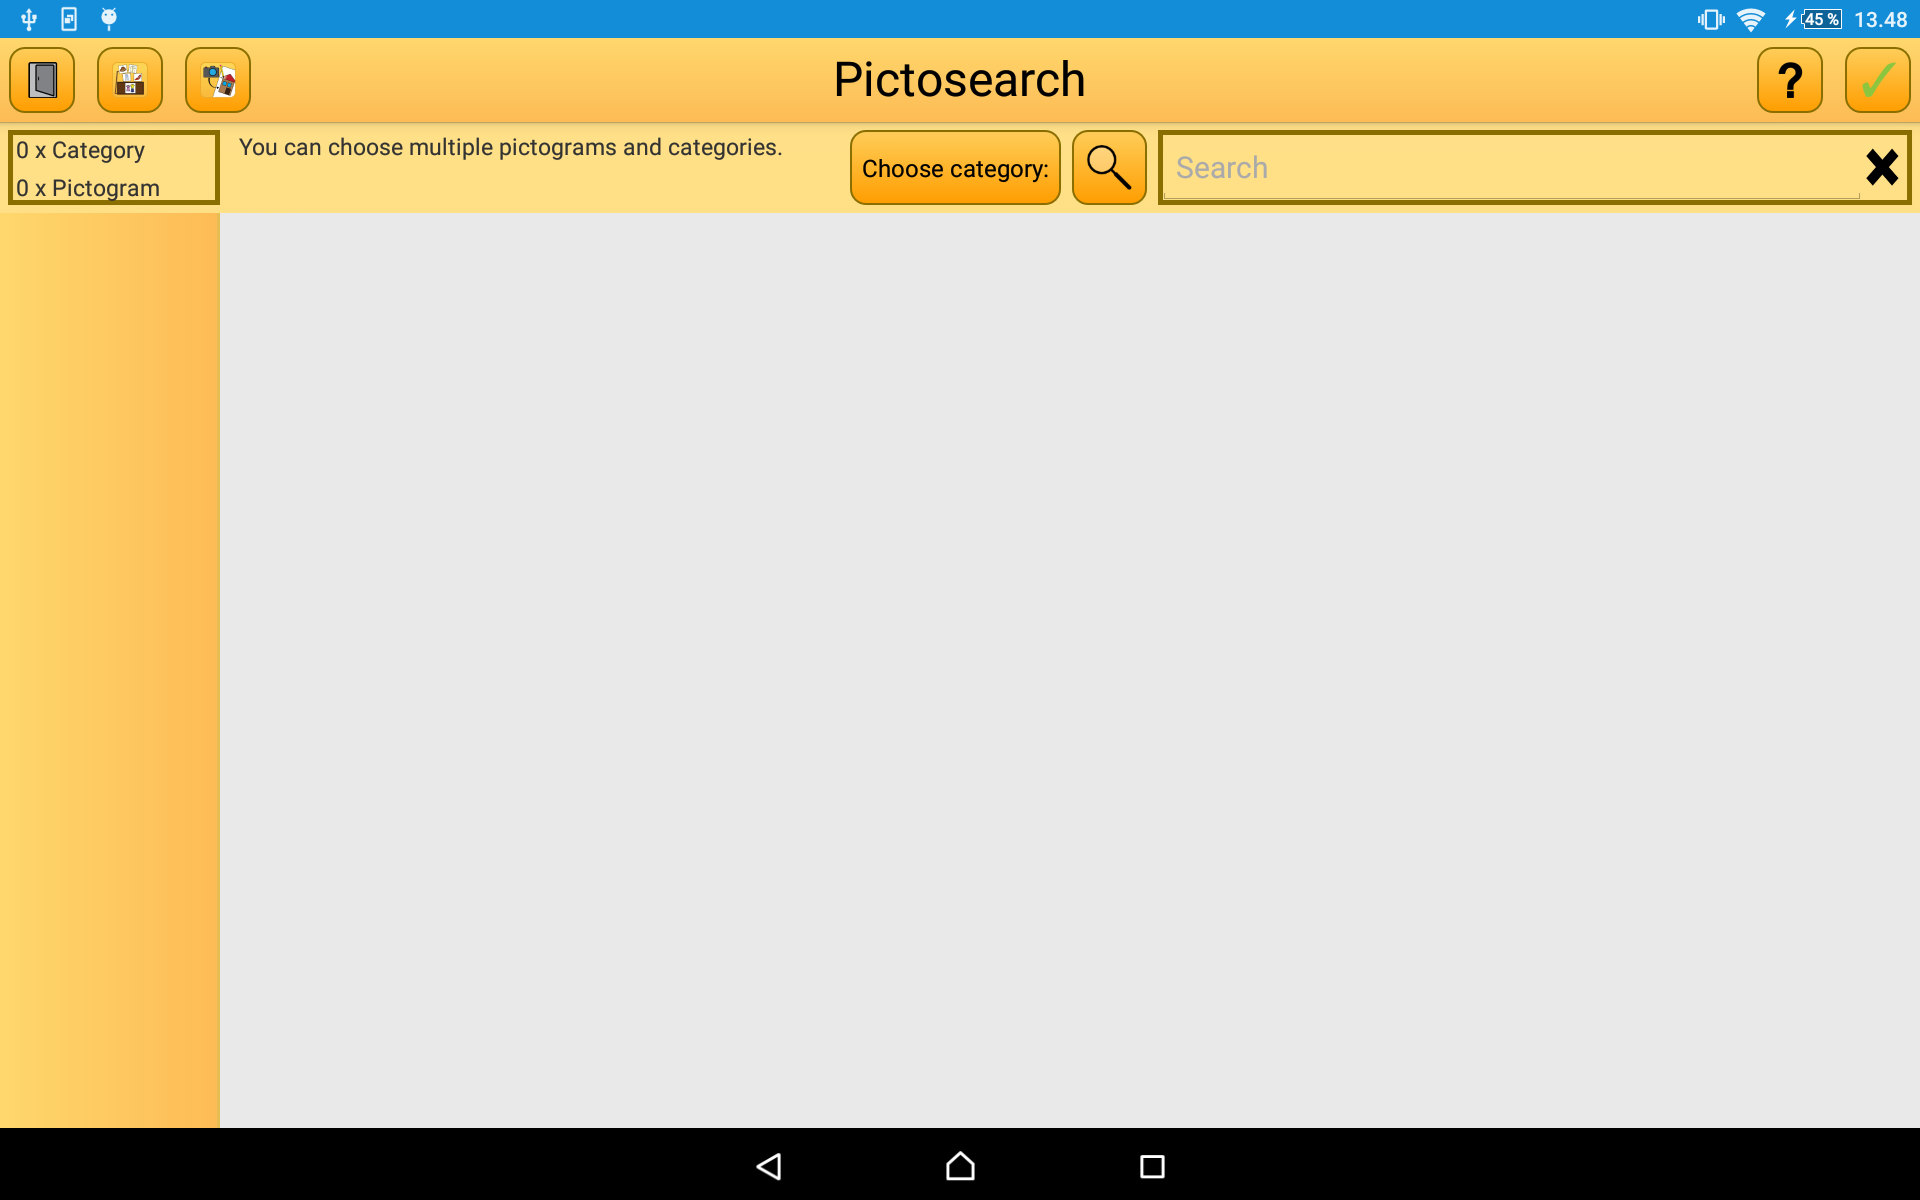
\includegraphics[width=0.8\textwidth]{images/old_startup.png}
                \end{figure}
                }

                \only<2| handout:2>{
                New view:
                \begin{figure}[htb]
                    \centering
                    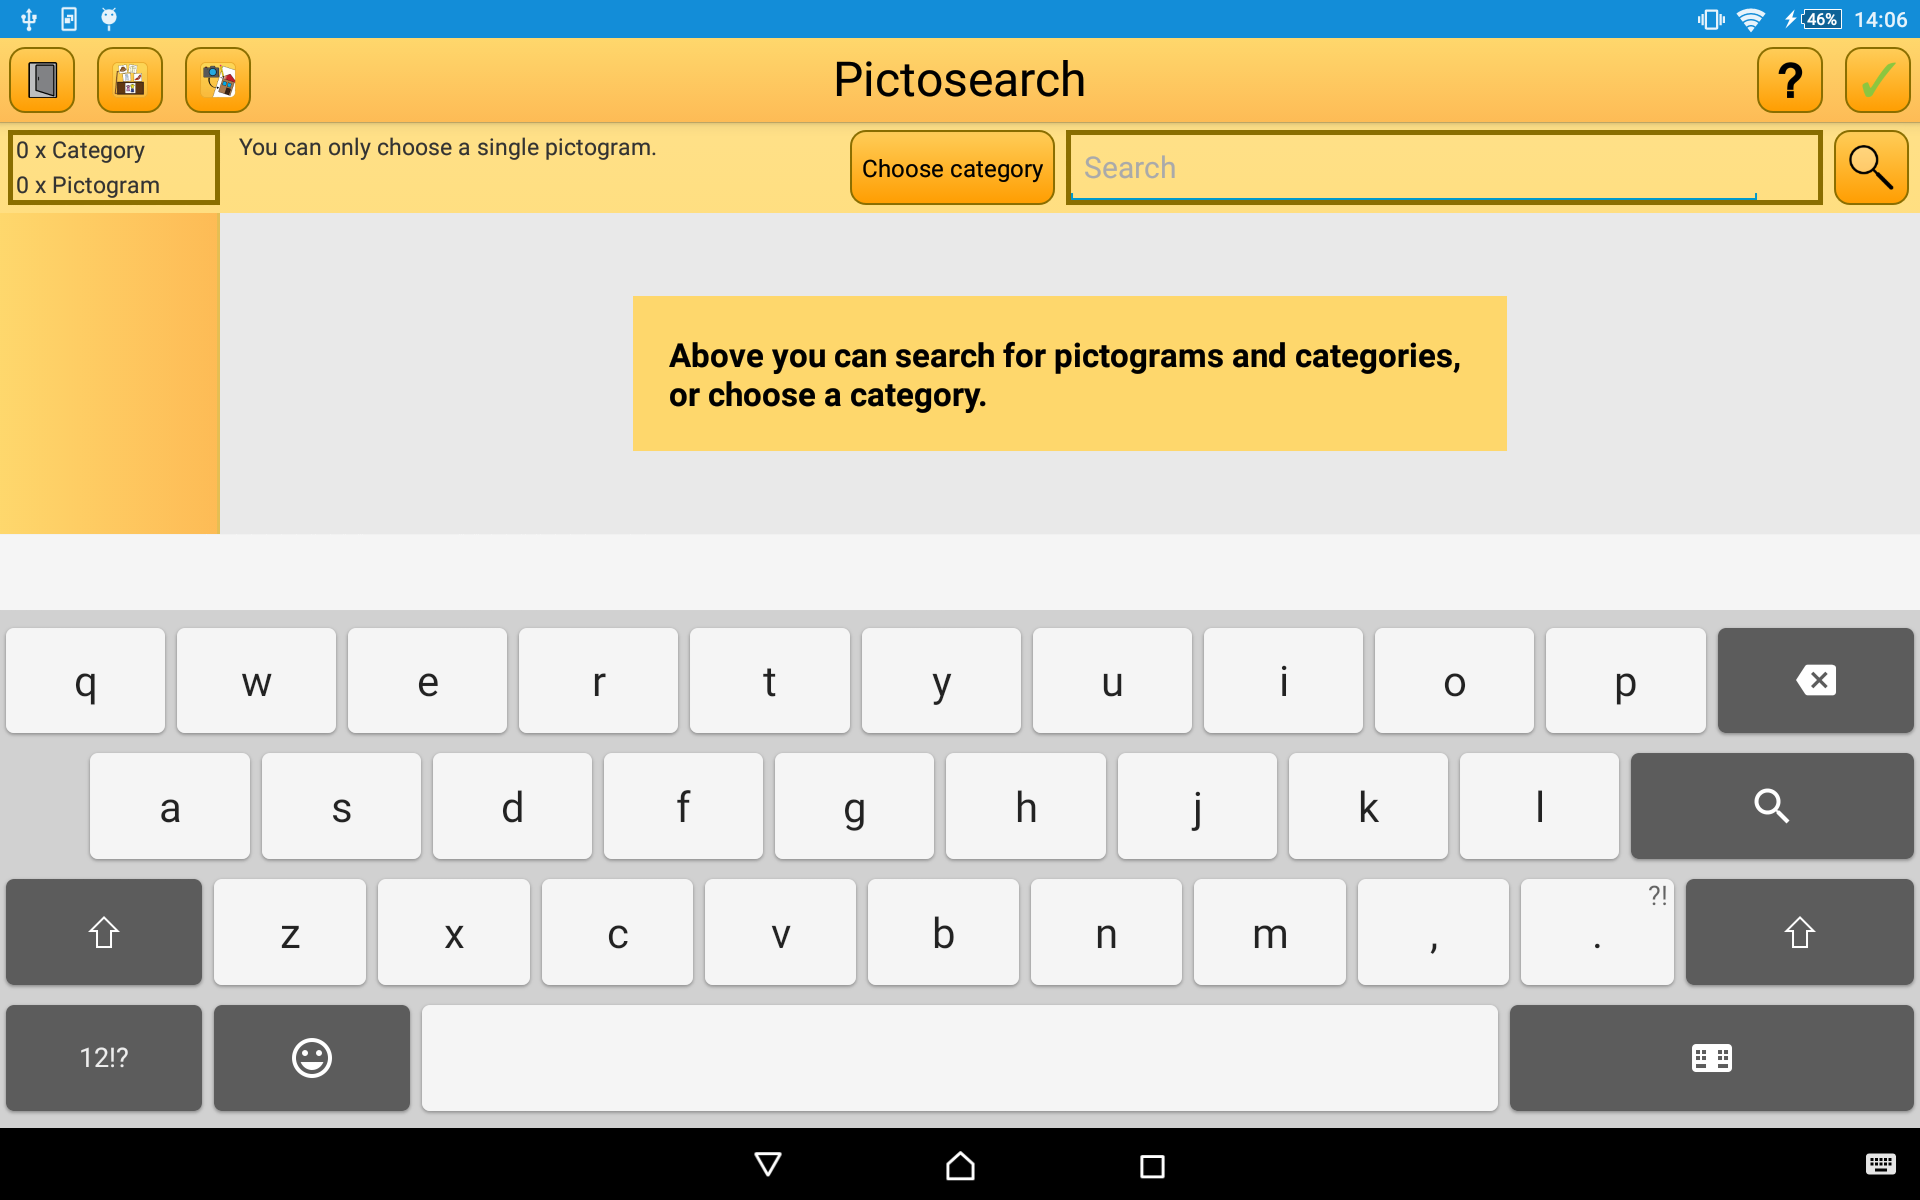
\includegraphics[width=0.8\textwidth]{images/new_startup.png}
                \end{figure}
                }

                \only<3| handout:3>{
                New view after typing the letter a:
                \begin{figure}[htb]
                    \centering
                    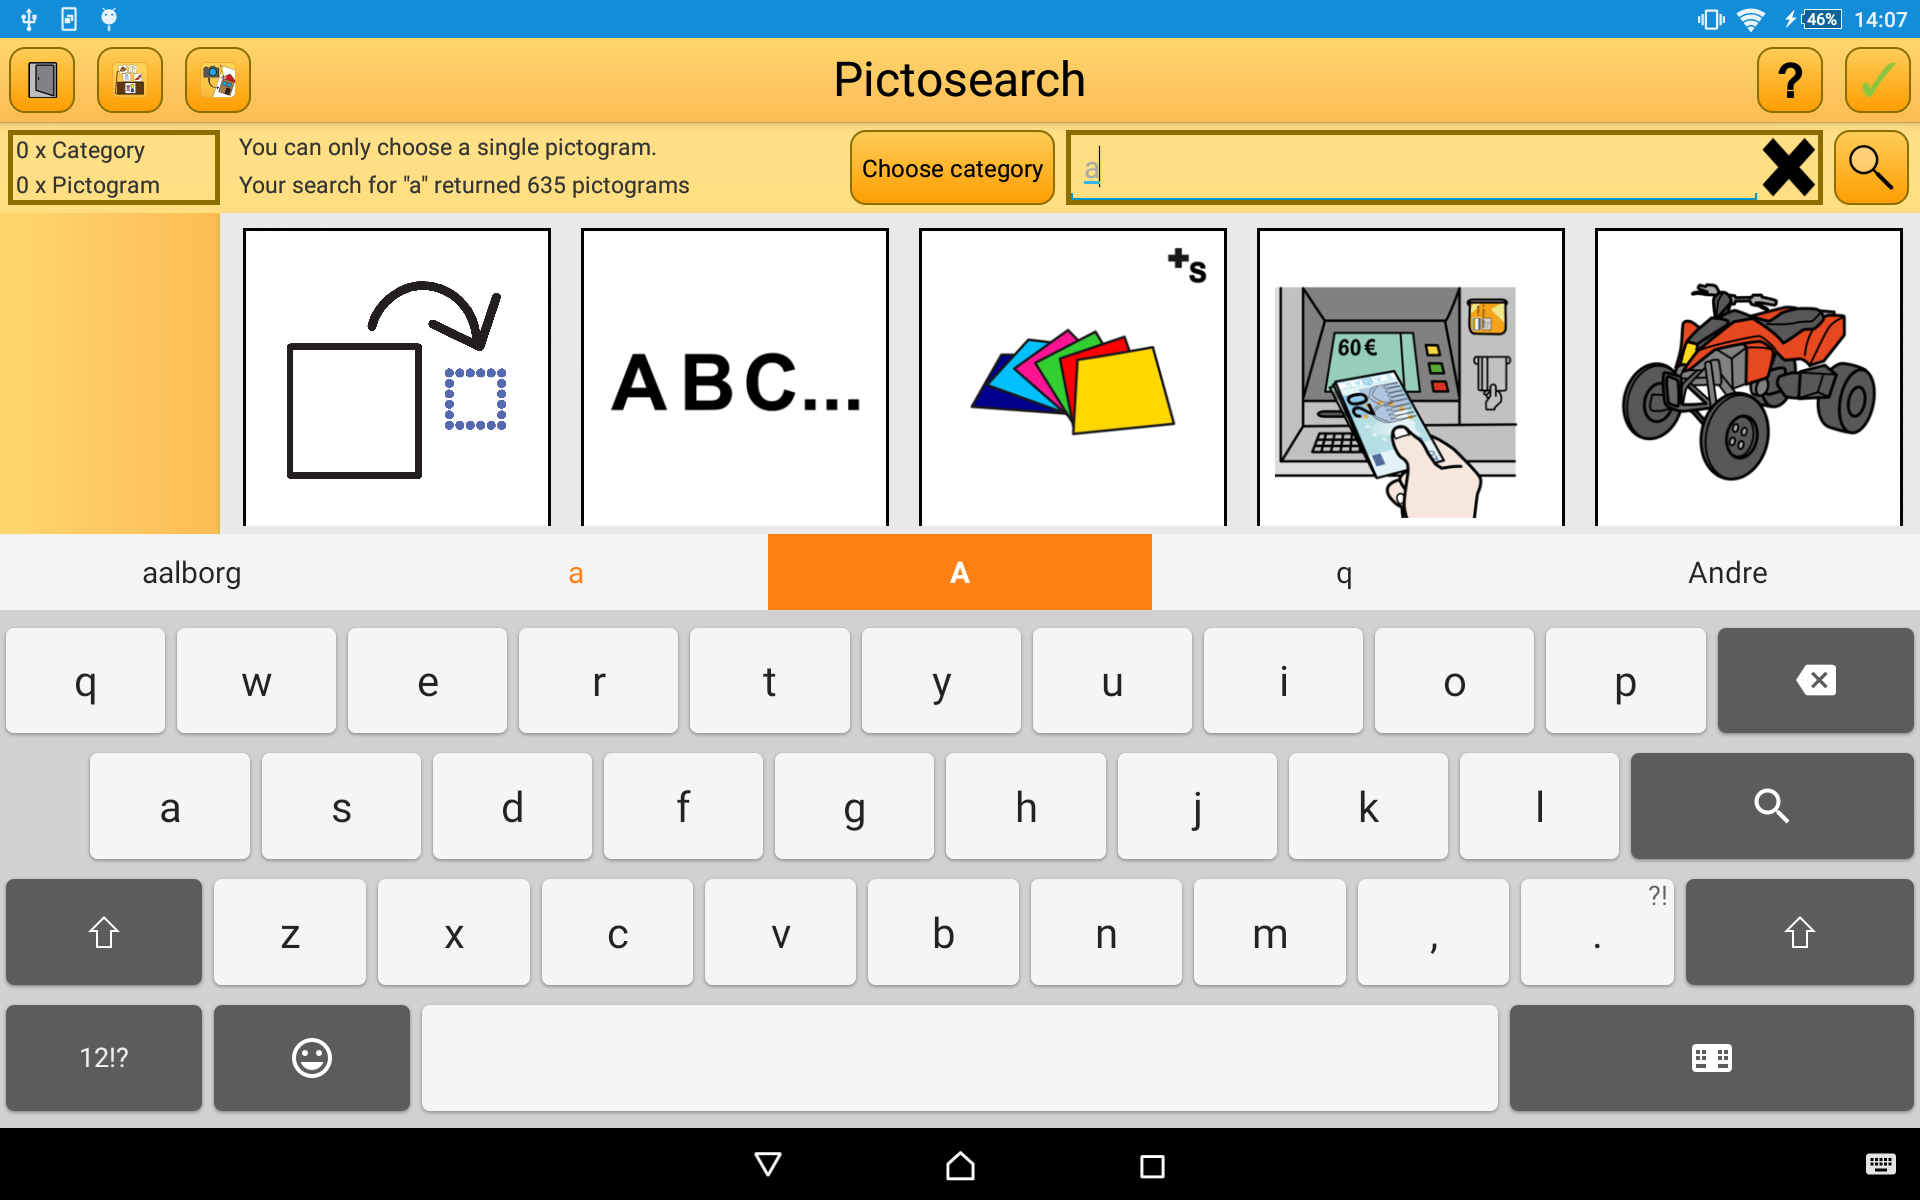
\includegraphics[width=0.8\textwidth]{images/new_searchresult.png}
                \end{figure}
                }
            \end{frame}

        \subsubsection{Week Schedule}
            \begin{frame}[t]{GIRAF--Apps}\framesubtitle{Week Schedule}
                \begin{itemize}
                    \item Added border to each frame.
                    \item Made the entire area scrollable.
                \end{itemize}
                \bigskip
                \only<1| handout:1>{
                Week Schedule example:
                \begin{figure}[htb]
                    \centering
                    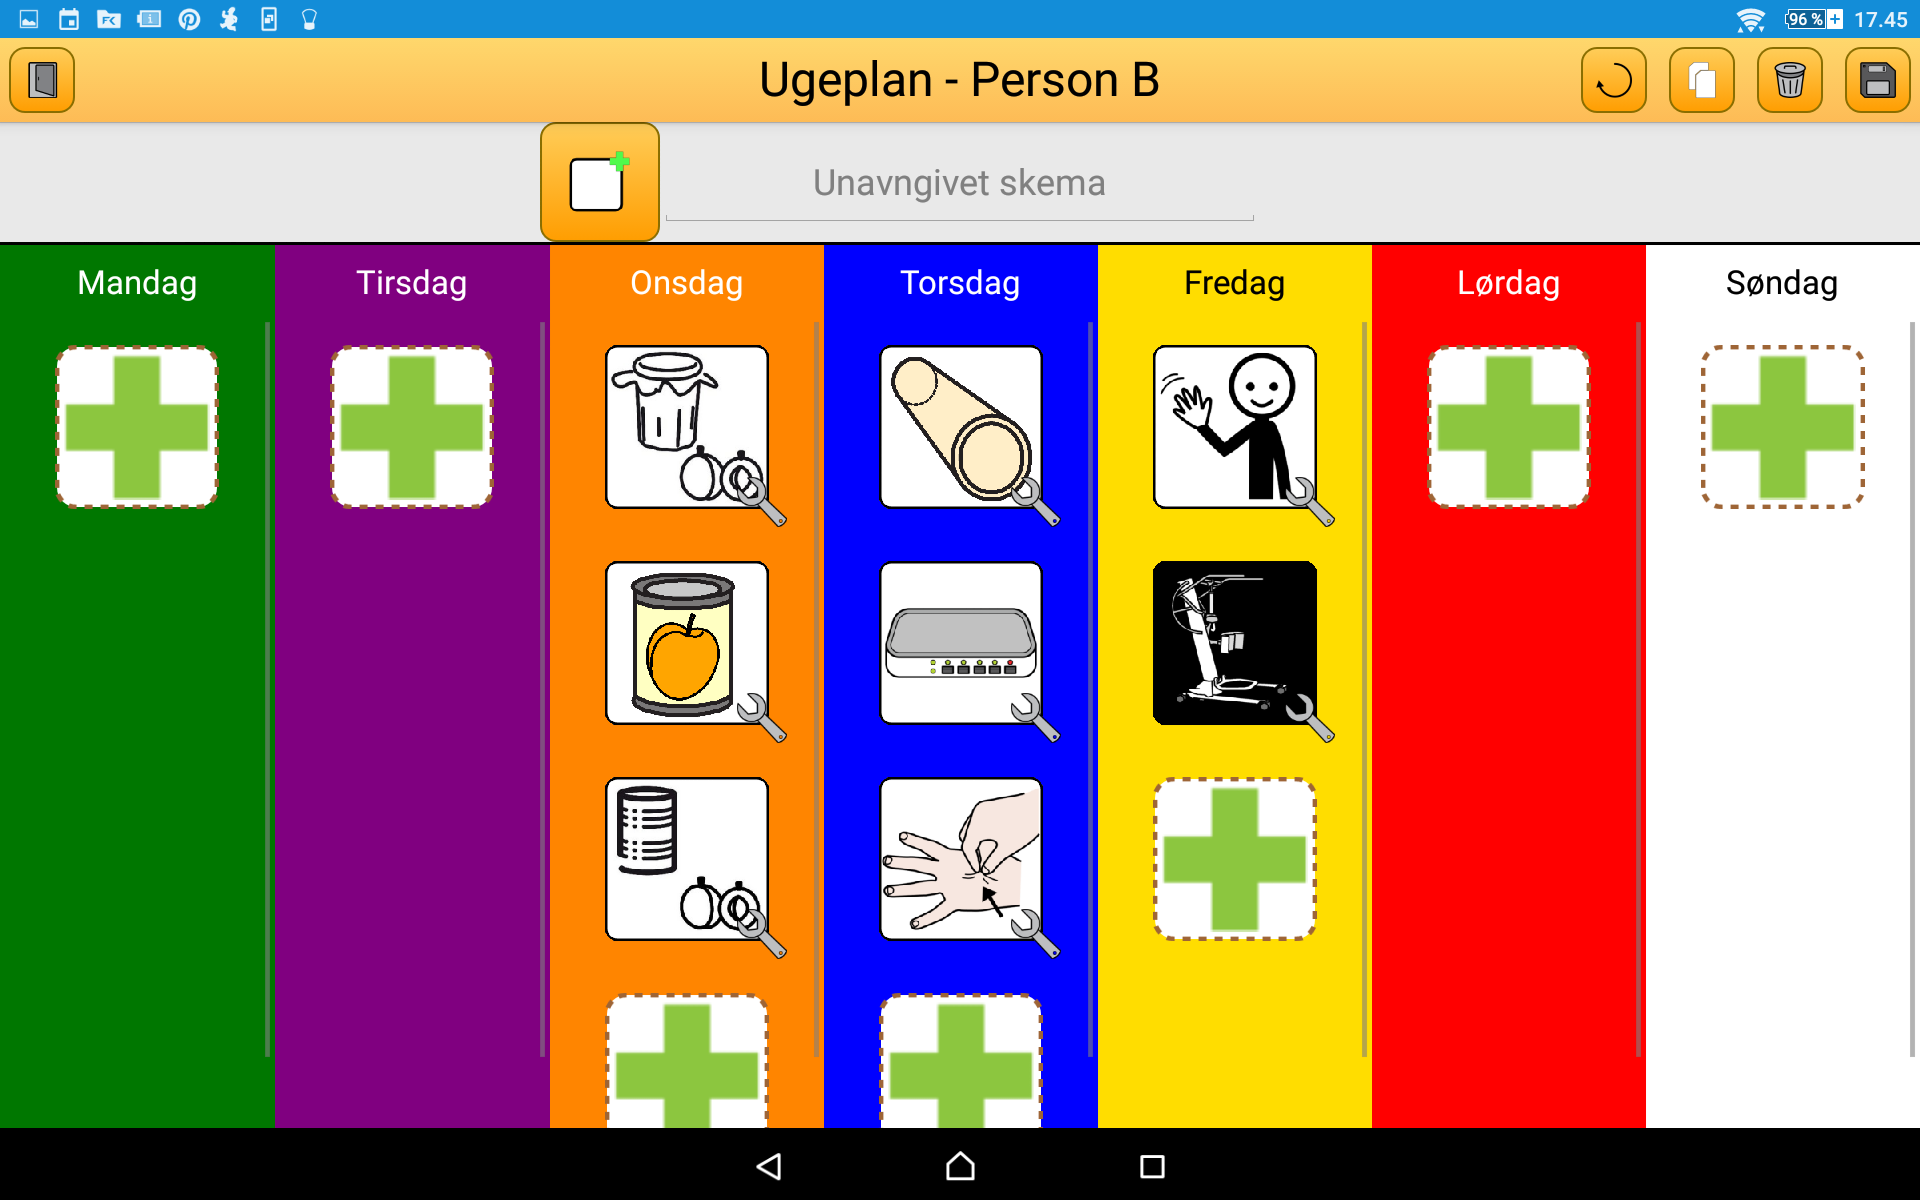
\includegraphics[width=0.8\textwidth]{images/ws_uden.png}
                \end{figure}
                }

                \only<2| handout:2>{
                Week Schedule example with layoutborders:
                \begin{figure}[htb]
                    \centering
                    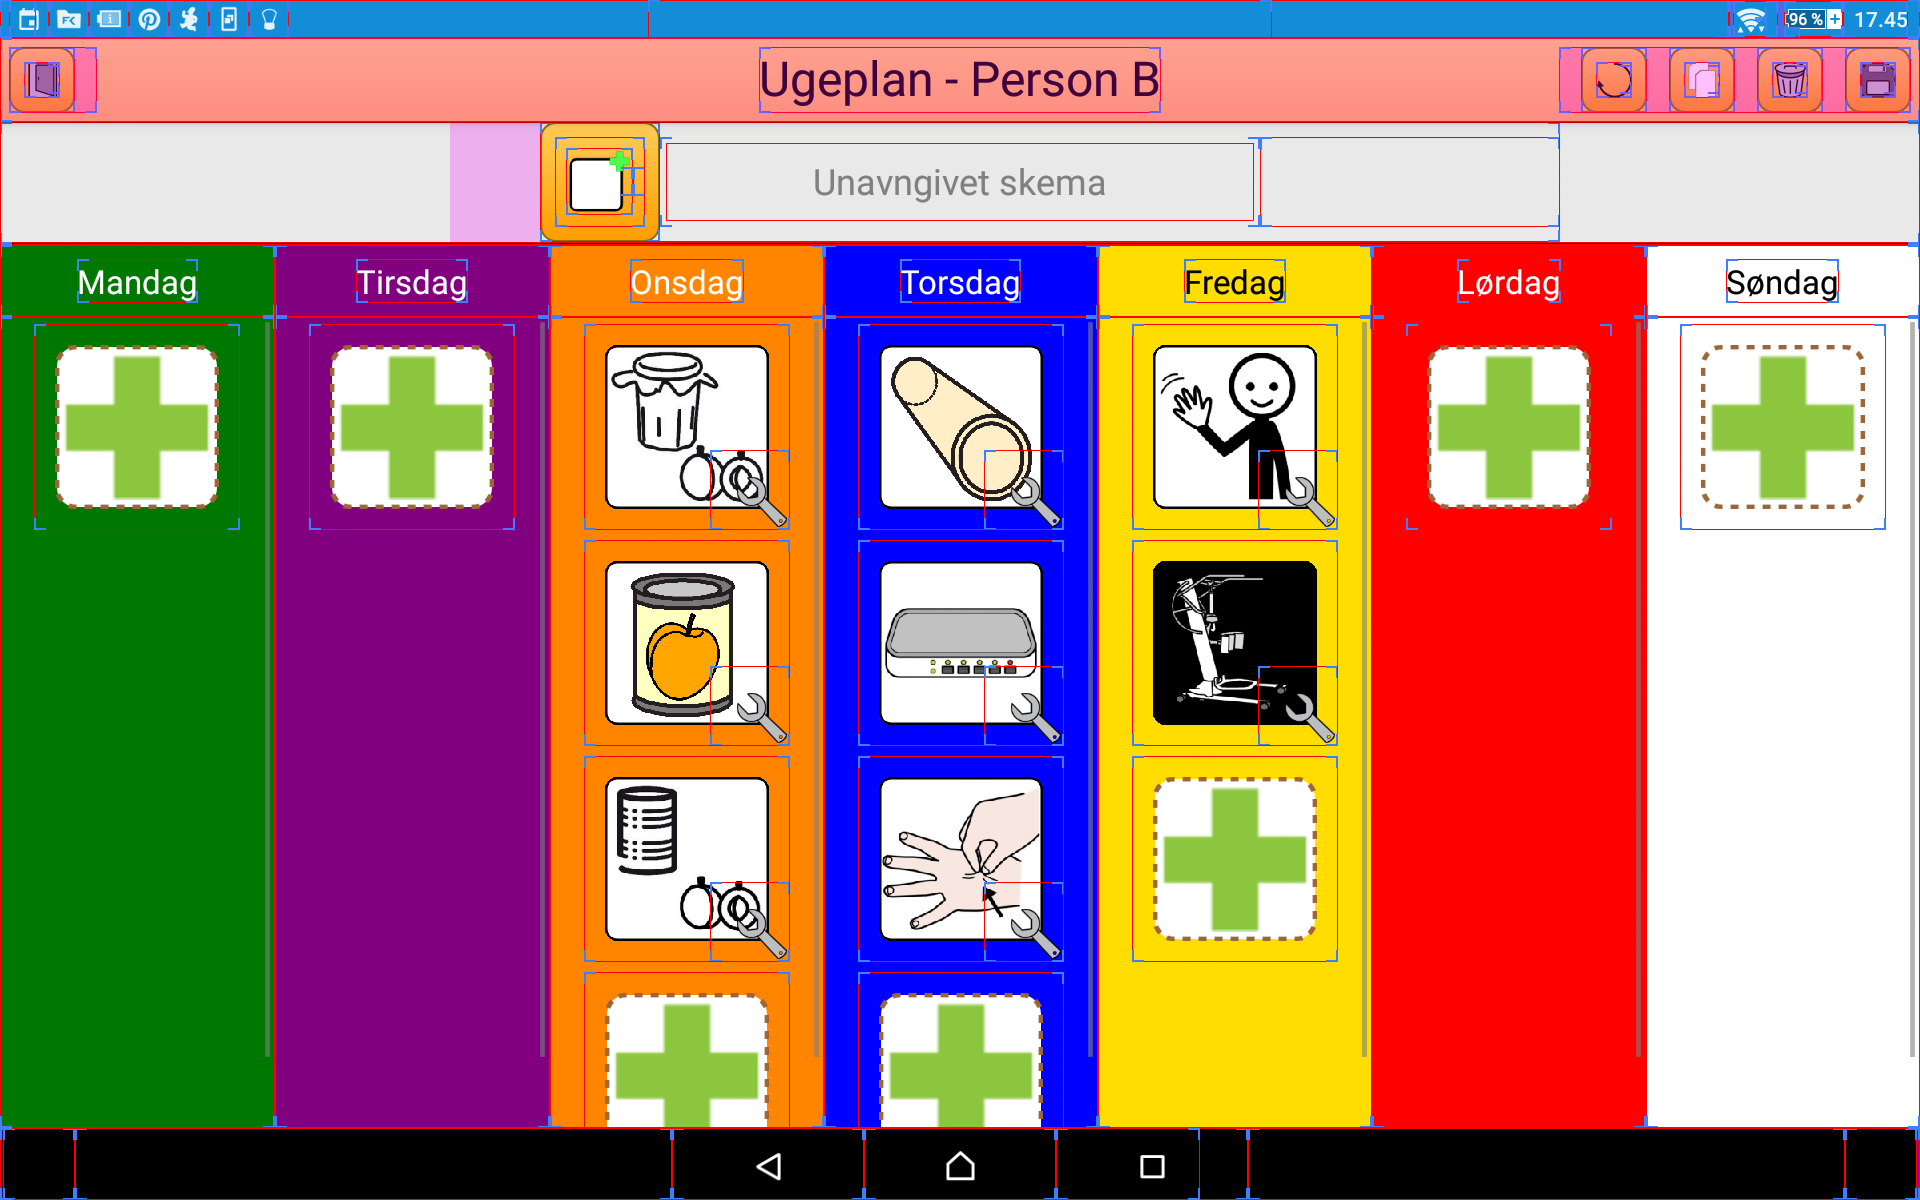
\includegraphics[width=0.8\textwidth]{images/ws_med.png}
                \end{figure}
                }


                \only<3| handout:3>{
                Week Schedule example with layoutborders zoomed:
                \begin{figure}[htb]
                    \centering
                    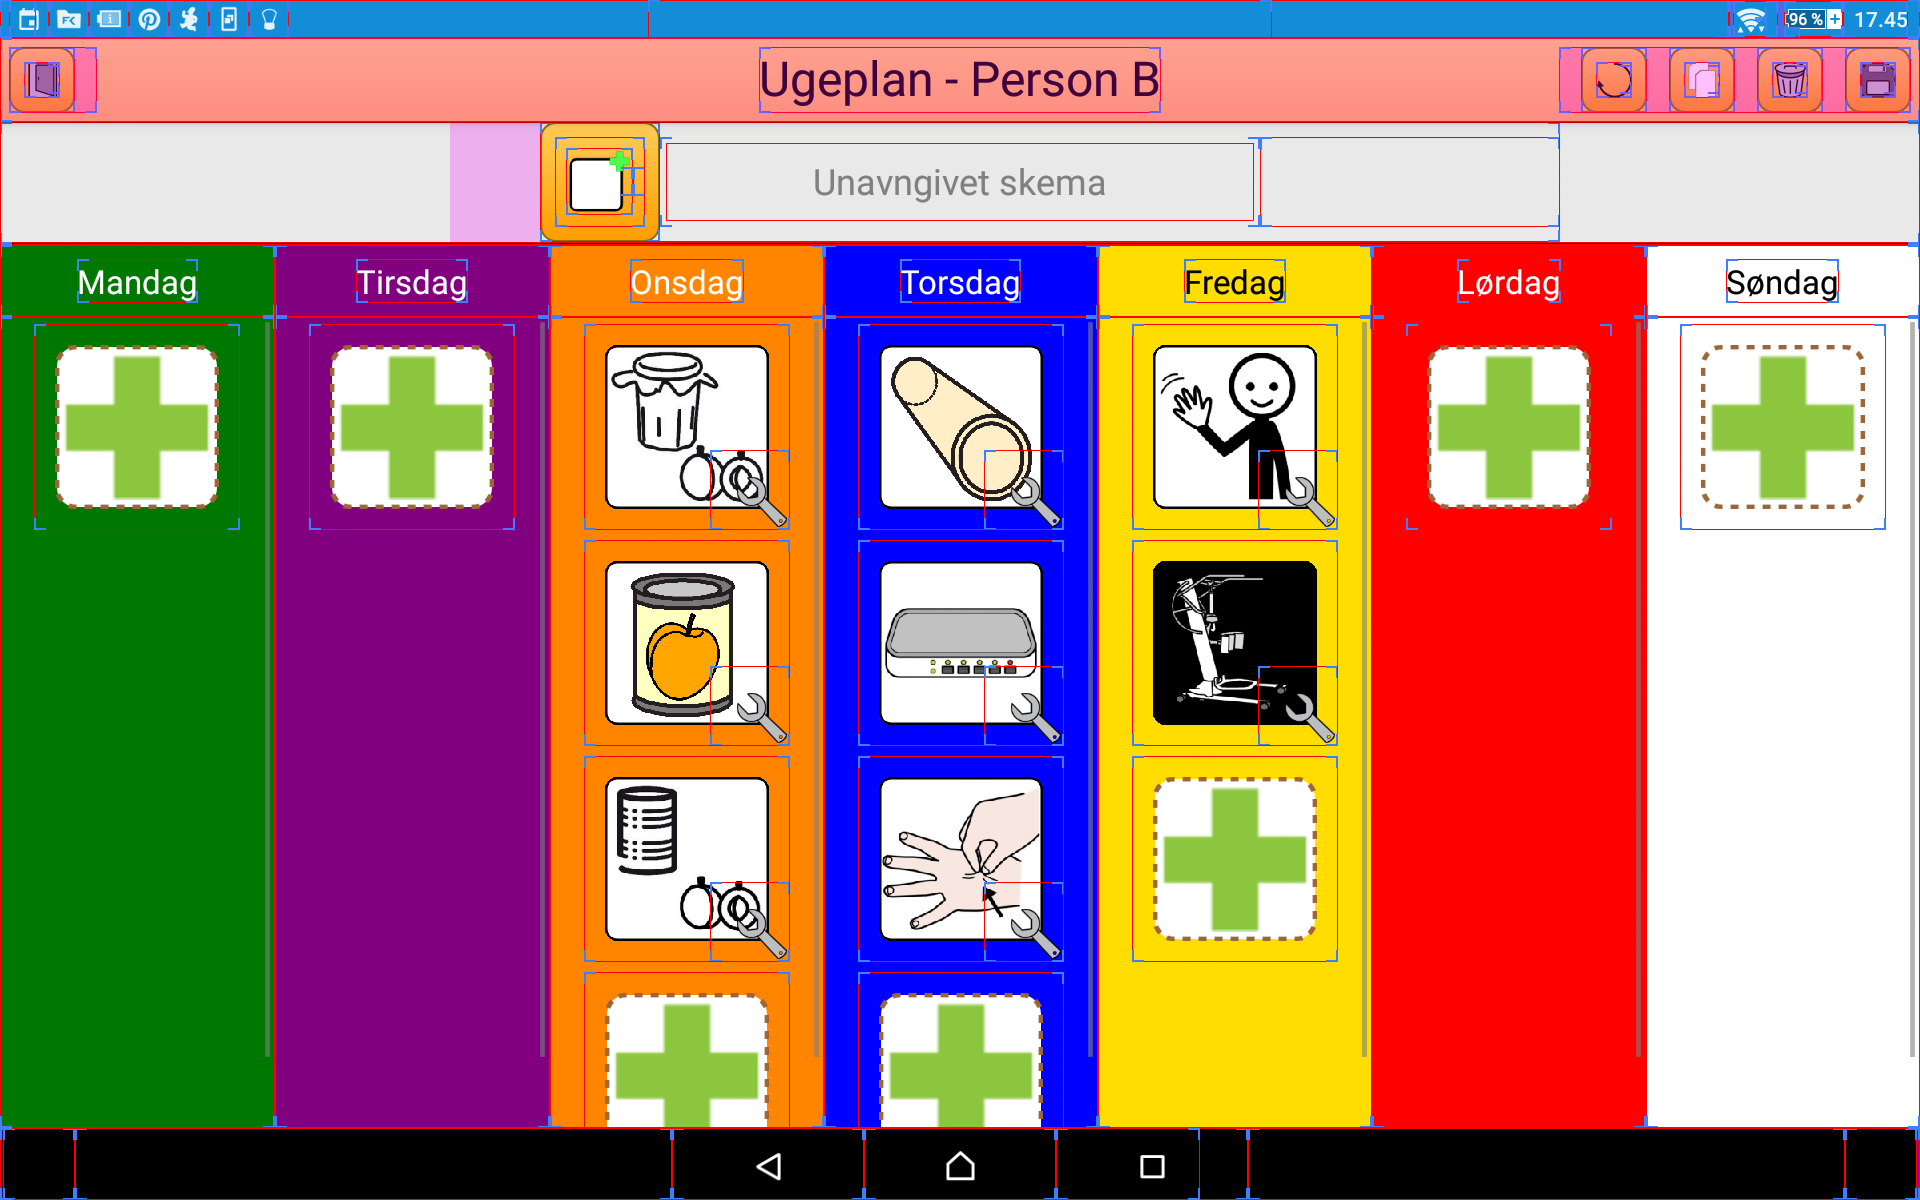
\includegraphics[trim={20cm 15.5cm 20cm 8.5cm},clip, width=0.8\textwidth]{images/ws_med.png}
                \end{figure}
                }

            \end{frame}
